\documentclass[fleqn]{article}

\usepackage{mydefs}
\usepackage{notes}
\usepackage{url}
\usepackage{amsmath}
\usepackage{graphicx}
\graphicspath{ {images/} }
\usepackage{verbatim}
\usepackage{subfig}
\usepackage[rightcaption]{sidecap}


\begin{document}
\lecture{Computer Vision}{Mini Project 02}
{Name:Abhay Doke {UID:29552668}}



\textbf{\huge 1.Hybrid Images}


Images Used for hybrid images:
\vspace{10 mm}


\includegraphics[width=0.4\textwidth]{j2.jpg}

\includegraphics[width=0.4\textwidth]{j3.jpg}

\newpage

Output Hybrid image:

\vspace{10 mm}
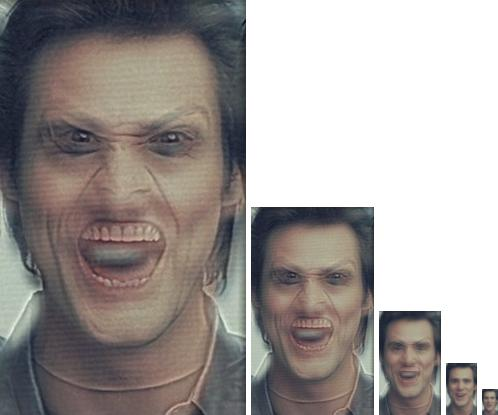
\includegraphics{jim_faces.jpg}
\vspace{10 mm}

For the Blurring, I used Sigma = 7 and for the Sharpening, Sigma = 5. 
\newpage
Code for making Hybrid Images:

\verbatiminput{hybridImage.m}



\newpage

\textbf{\huge 2. Photometric stereo}

\vspace{10 mm}
Code for \textbf{prepareData.m}

\verbatiminput{prepareData.m}


Code for \textbf{photometricStereo.m}

\verbatiminput{photometricStereo.m}


Code for \textbf{getSurface.m}

\verbatiminput{getSurface.m}

\newpage

Results for YaleB01:
 
\vspace{10 mm}
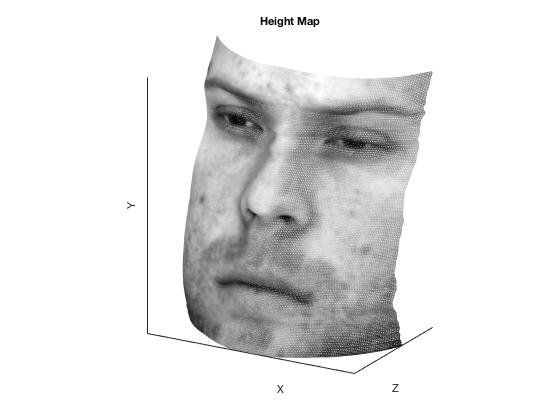
\includegraphics{yaleB01.jpg}
\newpage
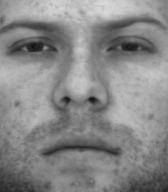
\includegraphics{yaleB01_albedo.jpg}

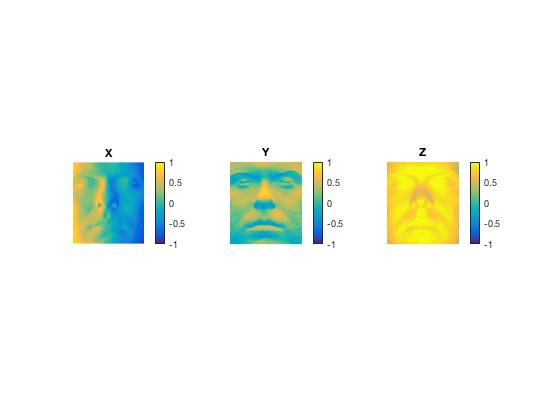
\includegraphics{a1.jpg}

\newpage

Results for YaleB02:
 
\vspace{10 mm}
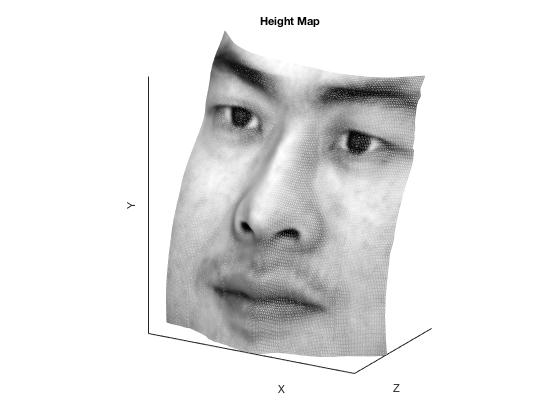
\includegraphics{yaleB02.jpg}
\newpage
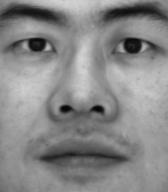
\includegraphics{yaleB02_albedo.jpg}

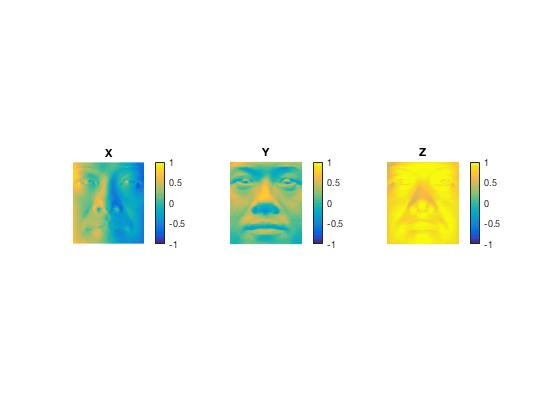
\includegraphics{a2.jpg}

\newpage

Results for YaleB05:
 
\vspace{10 mm}
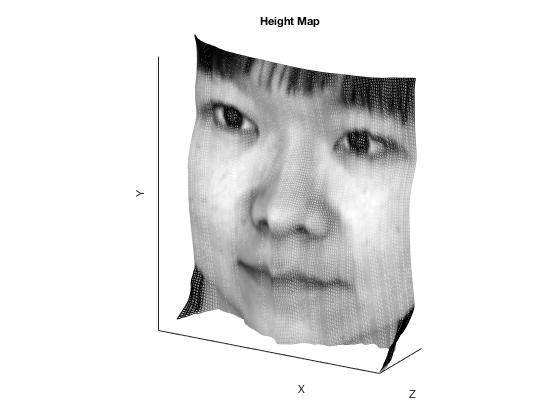
\includegraphics{yaleB05.jpg}
\newpage
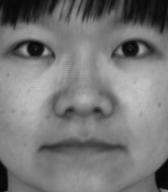
\includegraphics{yaleB05_albedo.jpg}

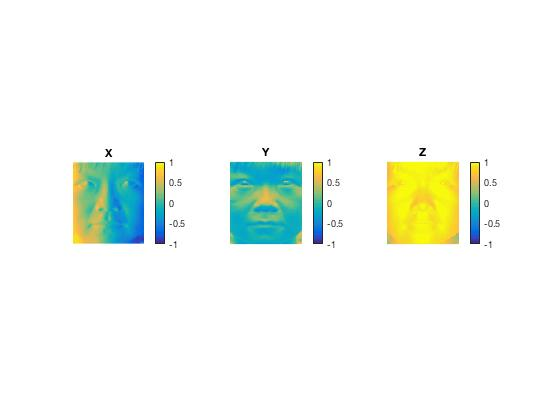
\includegraphics{a5.jpg}

\newpage

Results for YaleB07:
 
\vspace{10 mm}
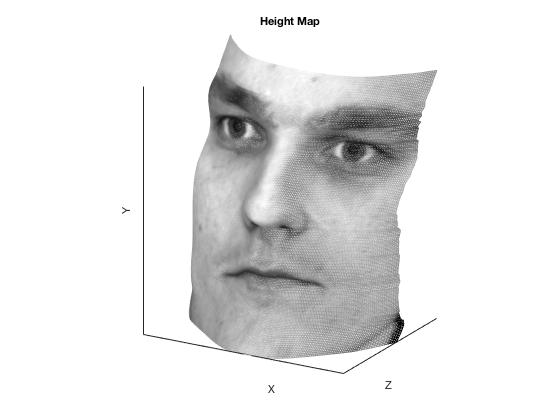
\includegraphics{yaleB07.jpg}
\newpage
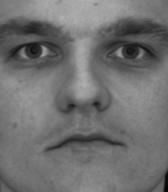
\includegraphics{yaleB07_albedo.jpg}

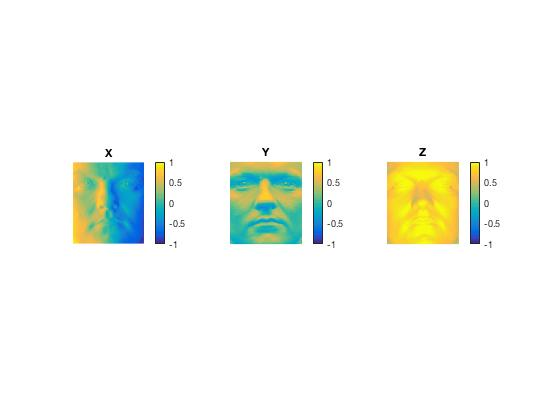
\includegraphics{a7.jpg}
\newpage
Difference between the integration methods for the yaleB02 subject.
\vspace{10 mm}

\begin{figure}[h]
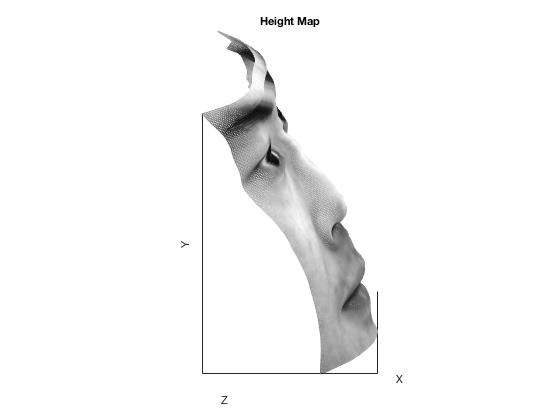
\includegraphics[width=0.5\textwidth]{ac copy.jpg}\caption{Integrating Columns and then Rows}
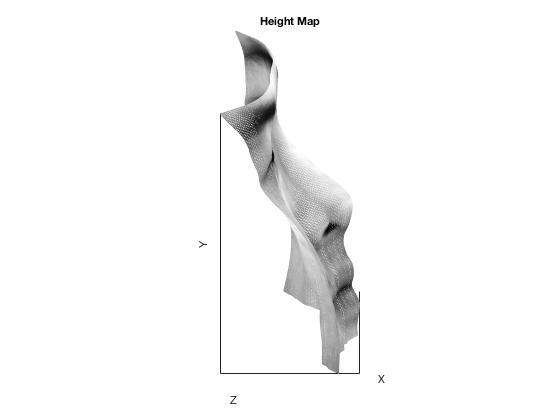
\includegraphics[width=0.5\textwidth]{ar copy.jpg}\caption{Integrating Rows and then Columns}
\end{figure}
\newpage
\begin{figure}[h]
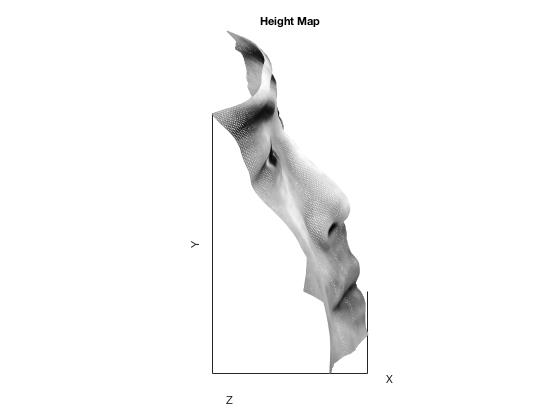
\includegraphics[width=0.5\textwidth]{aa copy.jpg}\caption{Average method }
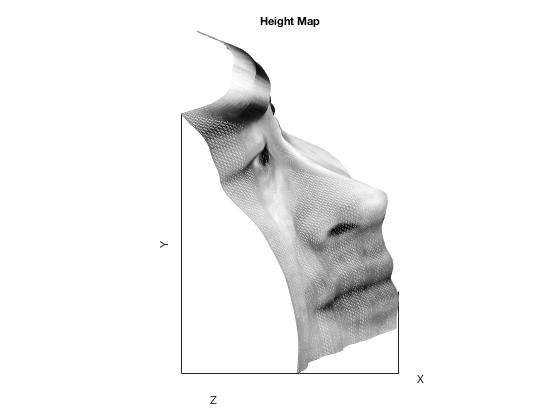
\includegraphics[width=0.5\textwidth]{aran copy.jpg}\caption{Random Method}
\end{figure}

\vspace{10 mm}
For the yaleB02 the average method works the best and the random method performs the worst.
Integrating with the column method makes the surface narrowed while integrating with the row method makes it more widened.
These effects can be resolved by using the average method.

Yale face data has shadow areas which violates assumptions of the shape-from shading method. Points which are in shadow affects the computation of the albedo image which in turns affects the computation of g(x, y).
This leads to false albedo points and also the surface depth gets affected and it becomes uneven.

\end{document}
